  \documentclass[a4paper,12pt]{report}

%Preambulo
\usepackage[portuguese]{babel}
\usepackage[utf8]{inputenc}
\usepackage{graphicx}
\graphicspath{ {images/} }
\usepackage{fancyhdr}
\usepackage{lastpage}
\usepackage{grffile}
\usepackage{color}
\usepackage{array}
\usepackage[dvipsnames]{xcolor}
\usepackage{courier}
\usepackage{indentfirst}
\usepackage{tcolorbox}
\usepackage{blindtext}
\usepackage{rotating}
\usepackage{tikz}
\usepackage{caption}



\title{\bf Projeto Sokoban \paragraph*{II FASE} }
\author{Francisco Oliveira \and Vitor Peixoto}
\date{20 Dezembro 2015 \\ \\ \\ \\ \\ \\ \\ \\ \\ \\ \\ \\ \\ \\ \\ \\  {\bf Laboratórios de Informática I \\ \\ Mestrado Integrado em Engenharia Informática}}



%Cabeçalho e Rodapé
\fancypagestyle{plain}{
	\fancyhf{}
	\fancyfoot[C]{Página \thepage\ de \pageref{LastPage}}
	\rhead{Laboratórios de Informática I - {\bf MIEI}}
	\lhead{2ª Fase - Projeto Sokoban}
	\renewcommand{\headrulewidth}{0.4pt}
	\renewcommand{\footrulewidth}{0.4pt}
}	
\pagestyle{fancy}
\fancyhf{}
\rhead{Laboratórios de Informática I - {\bf MIEI}}
\lhead{2ª Fase - Projeto Sokoban}
\renewcommand{\headrulewidth}{0.4pt}
\renewcommand{\footrulewidth}{0.4pt}
\fancyfoot[C]{Página \thepage\ de \pageref{LastPage}}
\definecolor{light-gray}{gray}{0.97}
%Estilo das Listings (Funções)
\lstset{
	backgroundcolor=\color{light-gray},
	frame=single,
	xleftmargin=2pt,
	stepnumber=1,
	breakatwhitespace=false,         
	breaklines=true, 
	numbers=left,
	numbersep=5pt,
	numberstyle=\ttfamily\tiny\color[gray]{0.20},
	belowcaptionskip=\bigskipamount,
	captionpos=b,
	escapeinside={*'}{'*},
	language=haskell,
	tabsize=4,
	emphstyle={\bf},
	commentstyle=\small\sc,
	stringstyle=\footnotesize\ttfamily,
	showspaces=false,
	columns=flexible,
	basicstyle=\footnotesize\ttfamily,
	keywordstyle=\footnotesize\ttfamily,
	showstringspaces=false,
	morecomment=[l]\%,
	tabsize=4
}
\renewcommand*{\lstlistlistingname}{Lista de Funções}




\begin{document}
\maketitle
\tableofcontents


\chapter{Introdução}

Este relatório foi realizado no âmbito da 2ª fase do projeto proposta na unidade curricular de Laboratórios de Informática I do Mestrado Integrado em Engenharia Informática. Foi-nos então proposto criar o jogo {\sl Sokoban}, que já havia sido trabalhado na 1ª fase deste mesmo projeto, na linguagem {\sl Haskell} em modo gráfico 2D usando como ferramenta a biblioteca {\sl Gloss}. 

Dada a sua utilidade para esta fase usamos funções de tarefas da 1ª fase, embora que ligeiramente modificadas e criamos outras funções de raiz, todas devidamente documentadas através da plataforma {\sl Haddock}.

Para chegarmos a resultados concretos adotamos uma postura que se baseia na aprendizagem através do erros. Tudo o que foi desenvolvido nas três tarefas que são explicadas neste relatório foi alcançado através de diversos erros e falhas que nos fizeram aprender o funcionamento da linguagem e as capacidades da biblioteca {\sl Gloss}.

Este relatório está orientado por quatro secções, onde será explorado os problemas a resolver, a nossa abordagem para as suas resoluções, os testes efetuados e por fim as conclusões que tiramos dos nossos erros e do resultado final em si.





\chapter{Descrição do Problema}

O ponto fulcral desta 2ª Fase do projeto está relacionado com o desenvolvimento do jogo {\sl Sokoban} de modo a podermos executar uma sequência de comandos até obtermos a vitória ou até esses comandos terem terminado, uma inicialização na biblioteca {\sl Gloss} e por fim a adaptação do jogo à biblioteca, com novas funcionalidades interessantes (como {\sl undo}, {\sl restart} e a seleção de vários níveis de jogo).

Para resolvermos este problema contamos com algumas funções importadas da 1ª Fase do projeto que serão úteis na medida em que auxiliam novas funções, contamos com o auxílio do {\it GlossExtras.hs}, podemos ainda obter ajuda em algumas explicações que são dadas quanto à utilização da biblioteca {\sl Gloss} em ficheiros disponíveis no {\sl Blackboard} e por fim, temos o sítio {\sf sokoban.info} para servir de guião ao visual do nosso jogo. Com o auxílio destas ferramentas podemos agora passar à resolução dos problemas propostos para estas três tarefas.

\begin{figure}[h]
	\centering
	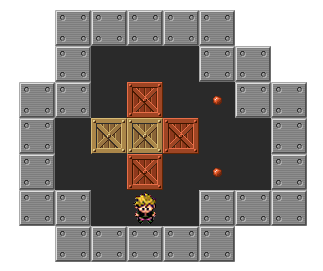
\includegraphics[width=0.4\textwidth]{image6}
	\caption{\small\sl Visual do jogo no sítio {\sf sokoban.info}}
	\captionsetup[figure]{list=yes}
\end{figure}





\chapter{Concepção da Solução}

\section{Tarefa D}

Esta tarefa será a responsável pela organização e sequencialização dos comandos. Assim, a biblioteca {\sl Gloss} ainda não será usada nesta tarefa computacional. Com efeito, como dito no enunciado do projeto, esta tarefa não será mais do que uma sequência de comandos efetuados em um só comando.
\\
\begin{lstlisting}[caption={\small\sl Função {\footnotesize\tt tarefa3'} que dado o tabuleiro, as coordenadas das caixas, do Sokoban e um movimento (U,D,L,R) devolve um par de inteiros com as novas coordenadas do Sokoban.\/}]
tarefa3' :: [String] -> [String]
tarefa3' tabuleiro = tarefa3Aux (reverse (funcaoPlantaMelhor tabuleiro)) (head (sepTabCOORDpares tabuleiro)) (last (init tabuleiro)) where 
	tarefa3Aux ((x:y):z) (a,b) direcáo 
		| direcao=="U" = movORnot ((x:y):z) (a,b) (0,1)
		| direcao=="D" = movORnot ((x:y):z) (a,b) (0,-1)
		| direcao=="L" = movORnot ((x:y):z) (a,b) (-1,0)
		| direcao=="R" = movORnot ((x:y):z) (a,b) (1,0)
		| otherwise = error "Comando nao aceite"
\end{lstlisting}

A função supradescrita será extremamente útil pois, usando como auxiliar nesta nova tarefa, será capaz de dar a nova coordenada do {\sl Sokoban} após um movimento. Ou seja, uma repetição desta função irá levar o {\sl Sokoban} a fazer a sequência de comandos inserida até chegar à vitória ou até os comandos terem terminado.

A função que executa o conjunto de comandos e devolve a resposta é a função {\footnotesize\tt tarefa4}. Nesta função é introduzido um tabuleiro com as coordenadas das caixas, do {\sl Sokoban} e as sequências de movimentos e devolve {\footnotesize\tt ["FIM <tick\_count>"] } caso as caixas estejam todas colocadas nos pontos, ou seja, o jogo esteja terminado, onde {\footnotesize\tt <tick\_count>} é o número de movimentos funcionais (aqueles em que o {\sl Sokoban} realmente moveu-se) efetuados, ou devolve {\footnotesize\tt ["INCOMPLETO <tick\_count>"] } caso as caixas não estejam todas colocadas nos pontos, ou seja, o jogo não esteja ainda acabado.
\\
\begin{lstlisting}[caption={\small\sl Função {\footnotesize\tt tarefa4} que dado o tabuleiro, as coordenadas das caixas, do Sokoban e uma sequência de movimentos ("UDLR" e.g.) devolve o estado do jogo e o número de movimentos funcionais efetuados.}]
tarefa4 :: [String] -> [String]
tarefa4 tabuleiro = rinceAndRepeat (tabuleiro) (last (init tabuleiro))
\end{lstlisting}

Esta função {\footnotesize\tt tarefa4} é auxiliada por muitas outras funções, sendo uma das mais relevantes a função {\footnotesize\tt vitoria} que deteta se ainda há algum carater {\footnotesize\tt H} no tabuleiro. Caso ainda haja algum carater {\tt H}, significa que o jogo ainda não está terminado. Esta função devolve {\footnotesize\tt "INCOMPLETO" }ou {\footnotesize\tt "FIM" }caso o jogo ainda não tenha terminado ou já tenha acabado, respetivamente. Esta função é chamada repetidamente na função {\footnotesize\tt rinceAndRepeat} (função semelhante à {\footnotesize\tt tarefa4}) para testar se a cada movimento que o {\sl Sokoban} faça ainda existe algum carater {\tt H}. Por isso é essencial uma função auxiliar que verifique se todas as caixas estão em cima de pontos.

Estas e outras mais funções, que podem ser visualizadas no módulo {\sl Haskell} "trabalhoD.hs" localizado no servidor {\sl SVN}, são essenciais para a funcionalidade desta tarefa.

Testes desta tarefa podem ser visualizados no capítulo Testes deste relatório.

\pagebreak







\section{Tarefa E}
A Tarefa E não tem como propósito efetuar desenvolvimentos no jogo, mas sim aperfeiçoar as nossas capacidades e habilidades com a biblioteca {\sl Gloss} através do tipo {\sl Picture}, um tipo que será fundamental na Tarefa F. O objetivo é determinar as dimensões do menor retângulo que envolve uma {\sl Picture}.

\begin{figure}[h]
	\centering
	
\includegraphics{image1}
	\caption{\small\sl Exemplo de retângulos de menores dimensões que envolve cada figura geométrica.}
	\captionsetup[figure]{list=yes}
\end{figure}

Neste caso, uma {\sl Picture} que ao ser criada ou ao sofrer modificações origine unicamente um píxel, deverá ser ignorada. As que originem realmente uma {\sl Picture} serão "admitidas" para uma lista formada unicamente por essa {\sl Picture}. 
\\
\begin{lstlisting}[caption={\small\sl Alguns exemplos da ação da função {\footnotesize\tt separadordePics} nas listas de Pictures.}]
separadordePics :: Picture -> [Picture]

-- Pictures que originam um ponto
separadordePics (Circle 0) = []
separadordePics (Scale 0 _ p) = []
separadordePics (Line []) = []

-- Pictures que nao originam um ponto
separadordePics (Circle f) = (Circle f):[]
separadordePics (Scale f1 f2 p) = (Scale f1 f2 p):[]
separadordePics (Line p) = (Line p):[]

-- Separacao da lista de Pictures
separadordePics (Pictures (p:[])) = (separadordePics p)
separadordePics (Pictures (p:t)) = (separadordePics p)++(separadordePics (Pictures t))
\end{lstlisting}

A função {\footnotesize\tt separadordePics} separa uma {\sl Picture} nos seus diversos componentes.

Após a {\sl Picture} ser separada nas diversas {\sl Pictures} que a formam, iremos usar a função que, recebendo as {\sl Pictures}, descobre o retângulo de menores dimensões que envolve essa mesma {\sl Picture} usando como suporte duas funções auxiliares, a função {\footnotesize\tt quaisSaoCantos} e a função {\footnotesize\tt kindaComplicated}. 

A função {\footnotesize\tt quaisSaoCantos} dada uma {\sl [Point]} que define o Polígono ou Linha devolve o retângulo de menores dimensões que envolve esse mesmo Polígono ou Linha.

A função {\footnotesize\tt kindaComplicated} é a função auxiliar da {\footnotesize\tt listadeCaixasdasPics} que é chamada apenas quando queremos calcular o retângulo de menores dimensões que envolve uma {\sl Picture} quando é sujeita a transformações, tais como {\footnotesize\tt Rotate}, {\footnotesize\tt Translate} ou {\footnotesize\tt Scale}. Esta função foi executada com sucesso para as transformaçãoes {\footnotesize\tt Translate} e {\footnotesize\tt Scale}, no entanto, não conseguimos que o {\sl output} no {\footnotesize\tt Rotate} fosse o esperado. 

Nos outros dois casos, {\footnotesize\tt Circle} e {\footnotesize\tt Bitmap} não há a necessidade de recorrer a qualquer função auxiliar, pois, no caso do {\footnotesize\tt Circle} é facil determinar o retângulo que envolve o círculo através do raio.

\begin{figure}[h]
	\centering
	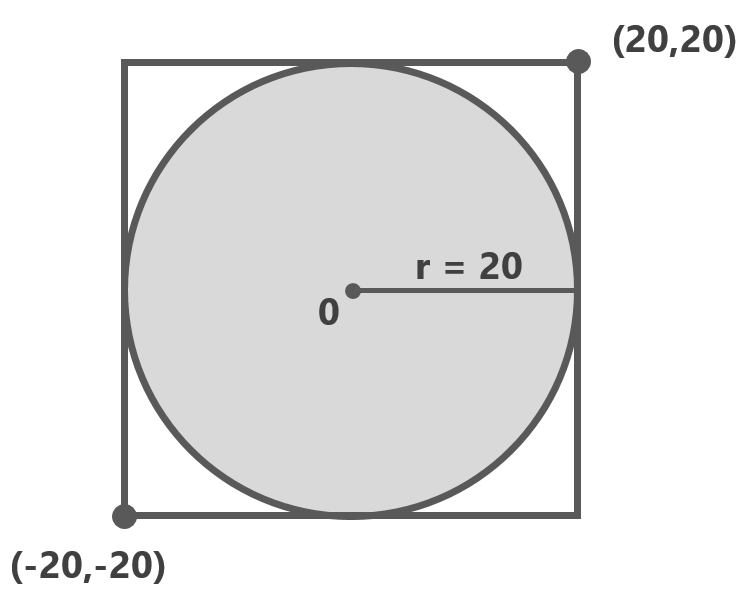
\includegraphics[width=0.4\textwidth]{image5}
	\caption{\small\sl O nosso método de cálculo das coordenadas do quadrado que envolve um círculo de raio 20.}
	\captionsetup[figure]{list=yes}
\end{figure}
No caso de um {\footnotesize\tt Bitmap}, como temos de introduzir a largura e comprimento que desejamos que esse {\footnotesize\tt Bitmap} tenha, apenas temos de passar de {\sl Int} para {\sl Float} usando a função predefinida {\footnotesize\tt fromIntegral} e definir as coordenadas do retângulo que envolve esse {\footnotesize\tt Bitmap}, sendo elas ((-w,-h),(w,h)). Sendo o "h" a altura e o "w" o comprimento, já em {\sl Float}.

No fim de calculadas as coordenadas que definem o retângulo somos agora obrigados a retribuir o output esperado para esta tarefa. Esse output será obtido através da função {\footnotesize\tt tarefa5}, uma função que devolve as dimensões do retângulo de menores dimensões que envolve cada {\sl Picture}. Para conseguirmos devolver as dimensões através das coordenadas das extremidades do retângulo, precisamos de duas funções auxiliares, a {\footnotesize\tt elCanto} e a {\footnotesize\tt elSize}.

A função {\footnotesize\tt elCanto} é a responsável por dizer qual são as coordenadas dos cantos que contém todas as outras coordenadas, ou seja, os pontos que se situam na coordenada mais distante da origem (0). Deste modo podemos obter o retângulo que envolve todas as {\sl Pictures} inicialmente introduzidas. 

A função {\footnotesize\tt elSize} é aquela que simplesmente transforma as coordenadas dos cantos do maior retângulo que envolve uma {\sl Picture} nas dimensões desse retângulo.

\begin{figure}[h]
	\centering
	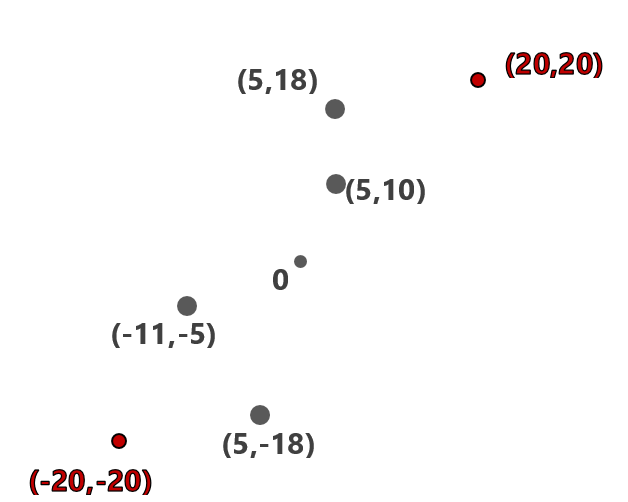
\includegraphics[width=0.6\textwidth]{image7}
	\caption{\small\sl Neste caso, as coordenadas dos cantos do maior retângulo que envolve todos os outros retângulos é ((-20,-20),(20,20)). A dimensão deste retângulo será de (40,40).}
	\captionsetup[figure]{list=yes}
\end{figure}

A função {\footnotesize\tt tarefa5} é nada menos do que a função que junta todos estas funções pela sua ordem sequencial correta:
\\
\begin{lstlisting}[caption={\small\sl Função {\footnotesize\tt tarefa5} que dada uma Picture que pode, ou não ser um conjunto de Pictures devolve o retângulo de menores dimensões que envolve essa Picture.}]
tarefa5 :: Picture -> (Int, Int)
tarefa5 pic = elSize (elCanto (listadeCaixasdasPics (separadordePics pic)))
\end{lstlisting}




\pagebreak













\section{Tarefa F}
Nesta tarefa iremos realmente criar o jogo {\sl Sokoban} recorrendo às capacidades gráficas da biblioteca {\sl Gloss}. Tendo em conta que o nosso ponto de partida seria inspirado no estilo do sítio {\sf sokoban.info} criamos um tema baseado no famoso jogo {\sl Super Mario Bros.} Para isso criamos diferentes {\it bitmaps} inspirados no visual gráfico do jogo, respeitando sempre a jogabilidade e coerência necessários para a execução do {\sl Sokoban}. Estes {\it bitmaps} têm geralmente uma dimensão de 40x40 e foram criados usando a ferramenta de desenho {\sl MSPaint}. Alguns exemplos podem ser vistos abaixo ou encontrados na sua totalidade na pasta {\sl "bmp" }do servidor {\sl SVN}.
\begin{figure}[h]
	\centering
	
\includegraphics[width=0.6\textwidth]{image2}
	\caption{\small\sl Alguns exemplos dos bitmaps usados no jogo. O Mario representa o jogador. A caixa com o ponto de interrogação representa uma caixa que não está em cima do ponto. E a moeda é o ponto onde devemos colocar a caixa.}
	\captionsetup[figure]{list=yes}
\end{figure}

Devemos então passar à inserção dos {\it bitmaps} no jogo, usando para isso o pacote {\it Graphics.Gloss.Data.Picture} que nos permite para além de inserir {\it bitmaps}, desenhar também linhas, círculos, polígonos, texto e efetuar modificações às {\sl Pictures}.
\\

\begin{lstlisting}[caption={\small\sl Ponto de entrada {\footnotesize\tt main} que carrega os diversos bitmaps e executa a função {\footnotesize\tt joga} e o type Estado.}]
type Estado = ([String],[Picture],String,Int,String)

main = do
	boxoff <- loadBMP "BOXOFF.bmp"
	boxon <- loadBMP "BOXON.bmp"
	ponto <- loadBMP "PONTO.bmp"
	(...)
	l9 <- loadBMP "L9.bmp"
	joga (tabuleiros,[boxoff,boxon,ponto,(...),l9],"",0,mapa0) desenhaJogo reageEvento
\end{lstlisting}

\begin{lstlisting}[caption={\small\sl Função {\footnotesize\tt joga}}]
joga :: Estado -> (Estado -> Picture) -> (Event -> Estado -> Estado) -> IO ()
joga tabuleiro desenha reage = play (FullScreen (1366,768))
(makeColorI 153 217 234 1) 90
tabuleiro desenha reage (\time estado -> estado)
\end{lstlisting}

A função {\footnotesize\tt joga} é a equivalente à função {\footnotesize\tt display} definida no pacote {\it Graphics.Gloss} e tem como função atualizar e desenhar a janela. Dado um tabuleiro e a lista das {\sl Pictures} \footnote{\scriptsize Sempre que esteja escrita a lista de {\sl Pictures} desta forma: {\scriptsize\tt [boxoff,boxon,ponto,(...),l9]} as reticências representam todos as outras {\sl Pictures} que foram ocultadas por questões de espaço. A lista completa seria: {\scriptsize\tt [boxoff,boxon,ponto,chao,parede,mario,undo,restart,sokoban,victory,help, l1,l2,l3,l4,l5,l6,l7,l8,l9,l0]} e deverá sempre ser entendido desta forma.} desenha o tabuleiro pedido ({\sl mapa0}; {\sl mapa1}; etc.) e atualiza o seu aspeto de acordo com os eventos introduzidos na função {\footnotesize\tt reageEvento}.

Esta janela vai estar em formato {\sl FullScreen} com a dimensão de (1366x768) píxeis. E terá uma cor de fundo à nossa escolha, que foi definida com o auxílio da função {\footnotesize\tt makeColorI} importada do pacote {\it Graphics.Gloss.Data.Color}. Sendo que o jogo não deverá sofrer alterações automaticamente com o passar do tempo, definimos a função anónima onde o tempo não é um fator influenciador do estado da janela: {\footnotesize\tt (time estado -> estado) }. Os mapas dos jogos estão definidos em funções com o seu respetivo nome. Estas funções são agrupadas numa lista na função {\footnotesize\tt tabuleiros}.
\\
\begin{lstlisting}[caption={\small\sl Função que define o {\footnotesize\tt mapa0} e função {\footnotesize\tt tabuleiros} que agrupa os mapas numa lista.}]
mapa0 :: String
mapa0 = outStr ["#######","#     #","#    .#","#    .#","#######","1 1","2 2","2 1",""]

tabuleiros :: [String]
tabuleiros = [mapa0,mapa1,(...),mapa9]
\end{lstlisting}

\pagebreak

\begin{figure}[h]
	\centering
	
\includegraphics[width=0.75\textwidth]{image3}
	\caption{\small\sl Seleção dos níveis (mapas) do jogo .}
	\captionsetup[figure]{list=yes}
\end{figure}
Para este jogo foram definidos 10 níveis com um grau de dificuldade geralmente crescente de acordo com os respetivos níveis. Os níveis são selecionados através de um clique na {\sl Picture} representativa do nível que queremos jogar ou através da tecla numérica correspondente ao número do nível.

O evento ocorrido após o clique do rato só é possível graças à função {\footnotesize\tt reageEvento}. Esta função efetua modificações no jogo através da introdução de comandos pelo teclado e/ou rato usando capacidades de um pacote extremamente útil da biblioteca {\sl Gloss}, {\it Graphics.Gloss.Interface.Pure.Game}.

\begin{lstlisting}[caption={\small\sl Excerto da função {\footnotesize\tt reageEvento}}]
-- Abre o Nivel 9
reageEvento :: Event -> Estado -> Estado
reageEvento (EventKey (MouseButton LeftButton ) (Down) (modifiers) (x,y)) (tabuleiro,[boxoff,boxon,ponto,(...),l9],moves,lvl,mapaatm)
		| ((x>=(205))&&(x<=(245))&&(y>=(((fromIntegral (length (funcaoPlantaMelhor (init (inStr mapaatm)))*(20)))+10)))&&(y<=((fromIntegral (length (funcaoPlantaMelhor (init (inStr mapaatm)))*(20)))+50))  ) = (tabuleiro,[boxoff,boxon,ponto,chao,parede,mario,undo,restart,sokoban,victory,help,l1,l2,l3,l4,l5,l6,l7,l8,l9,l0],moves,9,mapa0)
\end{lstlisting}

Neste excerto da função {\footnotesize\tt reageEvento} supradescrito, é chamado o construtor {\sl EventKey}, onde um clique com o botão esquerdo do rato ({\footnotesize\tt (MouseButton LeftButton)}) dentro da área da janela definida pelas coordenadas (x,y) provoca uma alteração em {\footnotesize\tt lvl}, um valor inteiro, que passa a ter o valor de 9. Este valor está localizado no {\sl type Estado}. A função {\footnotesize\tt joga} irá ser executada novamente, sofrendo uma alteração:
\begin{lstlisting}[caption={\small\sl A função {\footnotesize\tt joga}, que antes tinha o valor de 0, passa agora a ter o valor 9, fazendo com que apareça o mapa que escolhemos, o mapa9.}]
-- Antes
joga (tabuleiros,[boxoff,boxon,(...),l9],"",0,mapa0) desenhaJogo reageEvento

-- Depois
joga (tabuleiros,[boxoff,boxon,(...),l9],"",9,mapa9) desenhaJogo reageEvento
\end{lstlisting}

Assim, o construtor {\sl EventKey} será extremamente útil, pois vai ser através dele que iremos introduzir as alterações que queremos fazer no jogo. Os movimentos do {\sl Sokoban} são introduzidos relacionando a tecla que se preme e introduzindo uma {\sl String} com o carater responsável ao movimento do {\sl Sokoban} como foi feito na {\footnotesize\tt tarefa4} com "U", "D", "L" ou "R". Como demonstra o exemplo abaixo, ao carregar na tecla {\footnotesize\tt KeyDown} irá inserir um "D" na lista de {\footnotesize\tt moves}, levando o {\sl Sokoban} a descer uma posição para baixo.
\\
\begin{lstlisting}[caption={\small\sl Excerto da função {\footnotesize\tt reageEvento} que desloca o Sokoban uma posição abaixo.}]
-- Move para baixo
reageEvento (EventKey (SpecialKey KeyDown     ) (Down) (_)         (pos)) (tabuleiro,[boxoff,boxon,ponto,(...),l9],moves,lvl,mapaatm) = (tabuleiro,[boxoff,boxon,ponto,(...),l9],moves++"D",lvl,mapaatm)
\end{lstlisting}

Para além das ferramentas obrigatórias para o normal funcionamento deste jogo, foi também criada a possibilidade de fazer {\sl undo} e {\sl restart} ao jogo através do uso das teclas Z e X, respetivamente e também com clique numa {\sl Picture}.

Para o {\sl undo} funcionar basta retroceder um movimento na lista de {\footnotesize\tt moves}, para isso temos de recorrer à função predefinida {\footnotesize\tt init} que devolve todos os elementos da lista de {\footnotesize\tt moves} exceto o último, ou seja, remove o último movimento. Isto não se aplica caso ainda não tenha havido nenhum movimento, nesse caso, carregar na tecla 'Z' não irá provocar nenhum acontecimento. 

No caso do {\sl restart} apenas temos de dizer que a lista de {\footnotesize\tt moves} ainda não recebeu nenhum movimento, ou seja, uma lista vazia.
\\
\begin{lstlisting}[caption={\small\sl Excerto da função {\footnotesize\tt reageEvento} que é responsável por reiniciar a partida ou retroceder um movimento, usando as teclas X e Z.}]
-- Reinicia o jogo
reageEvento (EventKey (Char 'x')(Down)(_)(pos)) (tabuleiro,[boxoff,boxon,ponto,(...),l9],moves,lvl,mapaatm) = (tabuleiro,[boxoff,boxon,ponto,(...),l9],[],lvl,mapaatm)

-- Retrocede um movimento
reageEvento (EventKey (Char 'z')(Down)(_)(pos)) (tabuleiro,[boxoff,boxon,ponto,(...),l9],moves,lvl,mapaatm) = if (moves/=[]) 
then (tabuleiro,[boxoff,boxon,ponto,(...),l9],init moves,lvl,mapaatm)
else (tabuleiro,[boxoff,boxon,ponto,(...),l9],moves,lvl,mapaatm)   
\end{lstlisting}

O {\sl undo} e {\sl restart} é também executado, usando o clique do rato numa exata área. Essa área é definida da mesma forma que foi definida para a seleção de níveis e depois basta introduzir uma maneira de definir o {\sl output} exatamente igual à usada em cima. 

Assim sendo temos duas maneiras distintas de fazer {\sl undo} ou {\sl restart}.

\begin{figure}[h]
	\centering
	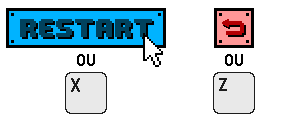
\includegraphics[width=0.56\textwidth]{image4}
	\caption{\small\sl Duas maneiras existentes de reiniciar a partida ou retroceder um movimento.}
	\captionsetup[figure]{list=yes}
\end{figure}

A função responsável por desenhar o mapa e outras {\sl Pictures} foi denominada de {\footnotesize\tt desenhaJogo}.

\begin{lstlisting}[caption={\small\sl Excerto da função {\footnotesize\tt desenhaJogo} que é responsável por desenhar as Pictures presentes na janela.}]
desenhaJogo :: Estado -> Picture
desenhaJogo (tabuleiro,[boxoff,boxon,ponto,(...),l9],moves,lvl,mapaatm) = 
	Pictures [ 
		-- Insere o mapa
		( Translate (fromIntegral (length (head (init (inStr mapaatm)))*(-20))) (fromIntegral (length (funcaoPlantaMelhor (init (inStr mapaatm)))*(-20))) (Pictures (desenhaJogoAux (reverse ( funcaoRemoveCard(tarefa4 ( (init (init (inStr mapaatm)))++[moves]++[""] ) )),[boxoff,boxon,ponto,(...),l9]) (0,0) ) ) ),
		-- Insere o bitmap "undo"
		(Translate (100) ((fromIntegral (length (funcaoPlantaMelhor (init (inStr mapaatm)))*(-20)))-40) undo),
		-- Insere o bitmap "restart"
		(Translate (-40) ((fromIntegral (length (funcaoPlantaMelhor (init (inStr mapaatm)))*(-20)))-40) restart),
		-- Insere o bitmap "sokoban"
		(Scale 1.1 1.1 (Translate (0) ((fromIntegral (length (funcaoPlantaMelhor (init (inStr mapaatm)))*(20)))+92) sokoban)),
		(...)
  
\end{lstlisting}

Esta função irá desenhar cada {\sl Picture} que queremos que apareça na janela. As {\sl Pictures} que ficam estáticas no jogo são de fácil inserção. Apenas temos de recorrer ao construtor {\footnotesize\tt Translate}, definir as coordenas X e Y da sua localização \footnote{\scriptsize A localização das {\sl Pictures}, em alguns casos, vai ser relativa ao tabuleiro, por isso calculamos o {\scriptsize\tt length} do mapa para podermos definir a localização (Y) da {\sl Picture} através da altura do mapa} e invocar a {\sl Picture} que queremos colocar naquela posição. Este processo pode ser visto no excerto supradescrito da mesma função.

Por outro lado, para inserir as {\sl Pictures} que formam o mapa na janela, o processo torna-se mais complicado. É também necessário recorrer ao construtor {\footnotesize\tt Translate}, mas neste caso as {\sl Pictures} que formam o mapa é composto por várias {\sl Pictures} e estão em constante mudança de acordo com os movimentos introduzidos na função {\footnotesize\tt reageEvento}. Assim, será necessário recorrer a uma função auxiliar, que recebe a {\footnotesize\tt tarefa4} com o mapa e os seus movimentos a serem dados na lista {\footnotesize\tt moves} e por fim com uma {\sl String} vazia concatenada ao mapa. É também dado à função auxiliar a lista de {\sl Pictures} que irão ser necessárias à construção do tabuleiro de jogo e um par de inteiros que indica que o mapa é desenhado a partir da coordenada (0,0), ponto a partir do qual todas as {\sl Pictures} que formam o mapa são desenhadas.
\\
\begin{figure}[h]
	\centering
	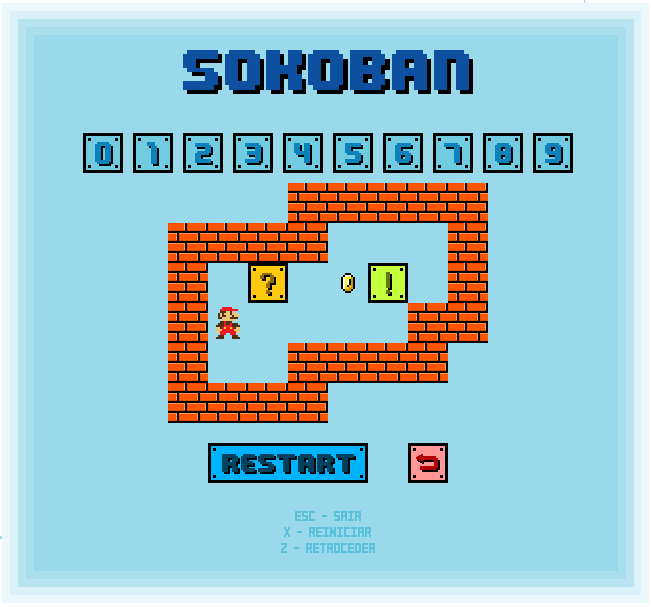
\includegraphics[width=0.7\textwidth]{image8}
	\caption{\small\sl Resultado final do jogo.}
	\captionsetup[figure]{list=yes}
\end{figure}











\chapter {Testes}

\section{Tarefa D}

Nesta secção são executados diversos testes à Tarefa D. Estes testes estão também disponíveis no servidor {\sl SVN} do nosso grupo de trabalho no formato ".txt" para serem executados, e provar a sua veracidade se necessário, na linha de comandos.
\\
\begin{tcolorbox}[width=\textwidth,colback={black},title={\sf Teste D.1:},outer arc=0mm,colupper=white]    
	{\footnotesize\tt *Main> tarefa4 ["\#\#\#\#\#","\#. .\#","\#   \#","\#   \#","\#\#\#\#\#","2 1","1 3","3 3","RU"," "]
		
		["FIM 0"] }
\end{tcolorbox} 

\begin{tcolorbox}[width=\textwidth,colback={black},title={\sf Teste D.2:},outer arc=0mm,colupper=white]    
	{\footnotesize\tt *Main> tarefa4 ["\#\#\#\#\#\#\#","\#     \#","\#    .\#","\#    .\#","\#\#\#\# \#\#\#","3 1","4 1","5 2","R",""]
		
		["FIM 1"] }
\end{tcolorbox} 

\begin{tcolorbox}[width=\textwidth,colback={black},title={\sf Teste D.3:},outer arc=0mm,colupper=white]    
	{\footnotesize\tt *Main> tarefa4 ["\#\#\#\#\#","\#. .\#","\#   \#","\#   \#","\#\#\#\#\#","2 1","1 2","3 2","RUDLLU"," "]
		
		["FIM 6"] }
\end{tcolorbox} 

\begin{tcolorbox}[width=\textwidth,colback={black},title={\sf Teste D.4:},outer arc=0mm,colupper=white]    
	{\footnotesize\tt *Main> tarefa4 ["\#\#\#\#\#","\#. .\#","\#   \#","\#   \#","\#\#\#\#\#","2 1","1 2","3 2","DDUDDDRUDLLU"," "]
		
		["FIM 8"] }
\end{tcolorbox} 

\begin{tcolorbox}[width=\textwidth,colback={black},title={\sf Teste D.5:},outer arc=0mm,colupper=white]    
	{\footnotesize\tt *Main> tarefa4 ["\#\#\#\#\#\#\#","\#     \#","\#    .\#","\#    .\#","\#\#\#\# \#\#\#","1 1","2 2","2 1","RRRUUULLLDRRR"," "]
		
		["FIM 12"] }
\end{tcolorbox}



\begin{tcolorbox}[width=\textwidth,colback={black},title={\sf Teste D.6:},outer arc=0mm,colupper=white]    
	{\footnotesize\tt *Main> tarefa4 ["\#\#\#\#\#","\#. .\#","\#   \#","\#   \#","\#\#\#\#\#","2 1","1 2","3 2","UURLLRDDRUDLLU"," "]
		
		["FIM 14"] }
\end{tcolorbox}

\begin{tcolorbox}[width=\textwidth,colback={black},title={\sf Teste D.7:},outer arc=0mm,colupper=white]    
	{\footnotesize\tt *Main> tarefa4 ["\#\#\#\#\#\#\#\#","\#\#\#\#   \#","\#   .. \#","\#     \#\#", "\#  \#\#\#\#\#","\#\#\#\# \#\#\#\#","4 4","3 3","4 3","DLDLLURRRURRDLDLLURLLLDDRULURR"," "]
		
		["FIM 30"] }
\end{tcolorbox}

\begin{tcolorbox}[width=\textwidth,colback={black},title={\sf Teste D.8:},outer arc=0mm,colupper=white]    
	{\footnotesize\tt *Main> tarefa4 ["\#\#\#\#\#\#","\#  \#\#\#","\#  \#\#\#","\#  \#\#\#","\#  \#\#\#", "\#.   \#","\#  . \#","\#  \#\#\#","\#\#\#\#\#\#","4 3","2 3","3 3", "DLLUUUDDDRRUULLDLURUULUURDDDDLDRUUULD"," "]
		
		["FIM 36"] }
\end{tcolorbox}

\begin{tcolorbox}[width=\textwidth,colback={black},title={\sf Teste D.9:},outer arc=0mm,colupper=white]    
	{\footnotesize\tt *Main> tarefa4 ["\#\#\#\#\#\#","\#  \#\#\#","\#  \#\#\#","\#  \#\#\#","\#  \#\#\#", "\#.   \#","\#  . \#","\#  \#\#\#","\#\#\#\#\#\#","4 3","2 3","3 3", "DDDUUULLLRRRRRRLLLUUUDDD"," "]
		
		["INCOMPLETO 3"] }
\end{tcolorbox}


\begin{tcolorbox}[width=\textwidth,colback={black},title={\sf Teste D.10:},outer arc=0mm,colupper=white]    
	{\footnotesize\tt *Main> tarefa4 ["\#\#\#\#\#\#\#\#","\#\#\#\#   \#","\#   .. \#","\#     \#\#", "\#  \#\#\#\#\#","\#\#\#\# \#\#\#\#","4 4","3 3","4 3","UUDLDR"," "]
		
		["INCOMPLETO 4"] }
\end{tcolorbox} 



\begin{tcolorbox}[width=\textwidth,colback={black},title={\sf Teste D.11:},outer arc=0mm,colupper=white]    
	{\footnotesize\tt *Main> tarefa4 ["\#\#\#\#\#","\#. .\#","\#   \#","\#   \#","\#\#\#\#\#","2 1","1 2","3 2","RUDLL"," "]
		
		["INCOMPLETO 5"] }
\end{tcolorbox} 

\begin{tcolorbox}[width=\textwidth,colback={black},title={\sf Teste D.12:},outer arc=0mm,colupper=white]    
	{\footnotesize\tt *Main> tarefa4 ["\#\#\#\#\#\#\#\#","\#\#\#\#   \#","\#   .. \#","\#     \#\#", "\#  \#\#\#\#\#","\#\#\#\# \#\#\#\#","4 4","3 3","4 3","DLLUDRR"," "]
		
		["INCOMPLETO 6"] }
\end{tcolorbox} 

\begin{tcolorbox}[width=\textwidth,colback={black},title={\sf Teste D.13:},outer arc=0mm,colupper=white]    
	{\footnotesize\tt *Main> tarefa4 ["\#\#\#\#\#\#","\#  \#\#\#","\#  \#\#\#","\#  \#\#\#","\#  \#\#\#", "\#.   \#","\#  . \#","\#  \#\#\#","\#\#\#\#\#\#","4 3","2 3","3 3", "DLLUUUU"," "]
		
		["INCOMPLETO 7"] }
\end{tcolorbox}

\begin{tcolorbox}[width=\textwidth,colback={black},title={\sf Teste D.14:},outer arc=0mm,colupper=white]    
	{\footnotesize\tt *Main> tarefa4 ["\#\#\#\#\#\#\#","\#     \#","\#    .\#","\#    .\#","\#\#\#\# \#\#\#","1 1","2 2","2 1","RRUULLDRR",""]
		
		["INCOMPLETO 9"] }
\end{tcolorbox} 






\section{Tarefa E}

Nesta secção são apresentados diversos testes à Tarefa E. Estes testes estão também disponíveis no servidor {\sl SVN} do nosso grupo de trabalho no formato ".txt" para serem executados, e provar a sua veracidade se necessário, na linha de comandos. No caso do Teste E.7 o resultado apresentado não é o correspondente ao que deveria ser na realidade. Devia dar (10,20) no entanto, como não conseguimos chegar a bom porto no que toca a este construtor, o resultado apresentado (0,0) não é o correto.
\\
\begin{tcolorbox}[width=\textwidth,colback={black},title={\sf Teste E.1:},outer arc=0mm,colupper=white]    
	{\footnotesize\tt *Main> tarefa5 (Line [(0,0),(20,0),(30,10),(20,20),(-30,0)])
		
		(60,20) }
\end{tcolorbox}

\begin{tcolorbox}[width=\textwidth,colback={black},title={\sf Teste E.2:},outer arc=0mm,colupper=white]    
	{\footnotesize\tt *Main> tarefa5 (Pictures [ Translate (-10) 0 (Circle 20), Translate 10 0 (Circle 15)])
		
		(55,40) }
\end{tcolorbox}

\begin{tcolorbox}[width=\textwidth,colback={black},title={\sf Teste E.3:},outer arc=0mm,colupper=white]    
	{\footnotesize\tt *Main> tarefa5 (Scale 2 3 (Line [(0,0),(20,0),(10,10),(0,0)]))
		
		(40,30) }
\end{tcolorbox}


\begin{tcolorbox}[width=\textwidth,colback={black},title={\sf Teste E.4:},outer arc=0mm,colupper=white]    
	{\footnotesize\tt *Main> tarefa5 (Translate 10 10 (Circle 15))
		
		(30,30) }
\end{tcolorbox}

\begin{tcolorbox}[width=\textwidth,colback={black},title={\sf Teste E.5:},outer arc=0mm,colupper=white]    
	{\footnotesize\tt *Main> tarefa5 (Circle 10)
		
		(20,20) }
\end{tcolorbox}

\begin{tcolorbox}[width=\textwidth,colback={black},title={\sf Teste E.6:},outer arc=0mm,colupper=white]    
	{\footnotesize\tt *Main> tarefa5 (Line [(0,0),(20,0),(10,10),(0,0)])
		
		(20,10) }
\end{tcolorbox}

\begin{tcolorbox}[width=\textwidth,colback={black},title={\sf Teste E.7:},outer arc=0mm,colupper=white]    
	{\footnotesize\tt *Main> tarefa5 (Rotate 90 (Line [(0,0),(20,0),(10,10),(0,0)]))
		
		(0,0) }
\end{tcolorbox}

\begin{tcolorbox}[width=\textwidth,colback={black},title={\sf Teste E.8:},outer arc=0mm,colupper=white]    
	{\footnotesize\tt *Main> tarefa5 (Translate 30 30 Blank)
		
		(0,0) }
\end{tcolorbox}

\begin{tcolorbox}[width=\textwidth,colback={black},title={\sf Teste E.9:},outer arc=0mm,colupper=white]    
	{\footnotesize\tt *Main> tarefa5 (Pictures [(Translate 10 10 (Circle 15)), (Scale 10 10 Blank),(Polygon [(10,20),(10,40),(30,40)])])
		
		(35,45) }
\end{tcolorbox}

\begin{tcolorbox}[width=\textwidth,colback={black},title={\sf Teste E.10:},outer arc=0mm,colupper=white]    
	{\footnotesize\tt *Main> tarefa5 (Scale 0 10 (Polygon [(10,20),(10,40), (30,40)]))
		
		(0,0) }
	
\end{tcolorbox}


\section{Tarefa F}

Nesta secção são apresentados diversos mapas criados para a Tarefa F. Estes testes estão também disponíveis no servidor {\sl SVN} do nosso grupo de trabalho no formato ".txt" para serem apenas visualizados. A sua execução é apenas possível através do módulo {\sl Haskell} "trabalhoF.hs" ou no executável "Sokoban.exe".

\begin{figure}[h]
	\centering
	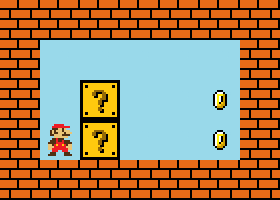
\includegraphics[width=0.25\textwidth]{teste0}
	\caption[]{\small\sl Teste F.1}
	\captionsetup[figure]{list=no}
\end{figure}

\begin{figure}[h]
	\centering
	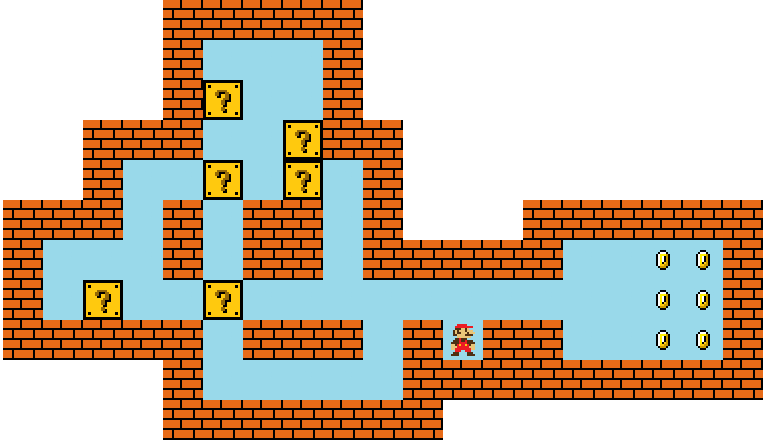
\includegraphics[width=0.65\textwidth]{teste1}
	\caption[]{\small\sl Teste F.2}
	\captionsetup[figure]{list=no}
\end{figure}

\begin{figure}[h]
	\centering
	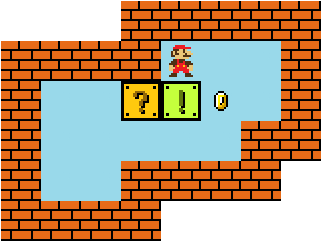
\includegraphics[width=0.30\textwidth]{teste2}
	\caption[]{\small\sl Teste F.3}
	\captionsetup[figure]{list=no}
\end{figure}

\begin{figure}[h]
	\centering
	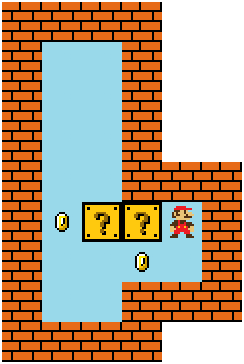
\includegraphics[width=0.225\textwidth]{teste3}
	\caption[]{\small\sl Teste F.4}
	\captionsetup[figure]{list=no}
\end{figure}

\begin{figure}[h]
	\centering
	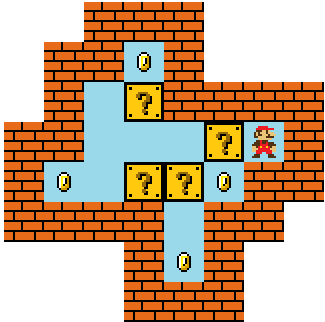
\includegraphics[width=0.29\textwidth]{teste4}
	\caption[]{\small\sl Teste F.5}
	\captionsetup[figure]{list=no}
\end{figure}

\begin{figure}[h]
	\centering
	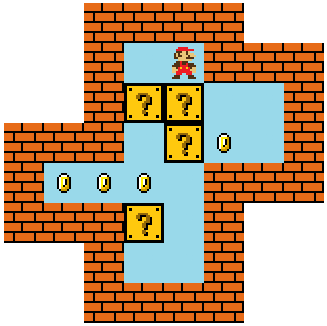
\includegraphics[width=0.29\textwidth]{teste5}
	\caption[]{\small\sl Teste F.6}
	\captionsetup[figure]{list=no}
\end{figure}

\begin{figure}[h]
	\centering
	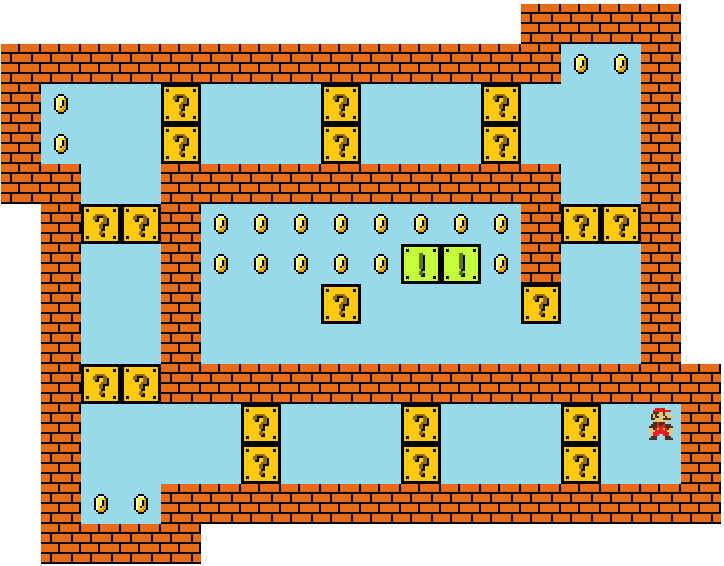
\includegraphics[width=0.64\textwidth]{teste6}
	\caption[]{\small\sl Teste F.7}
	\captionsetup[figure]{list=no}
\end{figure}

\begin{figure}[h]
	\centering
	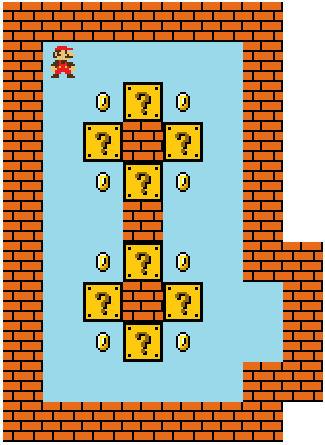
\includegraphics[width=0.317\textwidth]{teste7}
	\caption[]{\small\sl Teste F.8}
	\captionsetup[figure]{list=no}
\end{figure}

\begin{figure}[h]
	\centering
	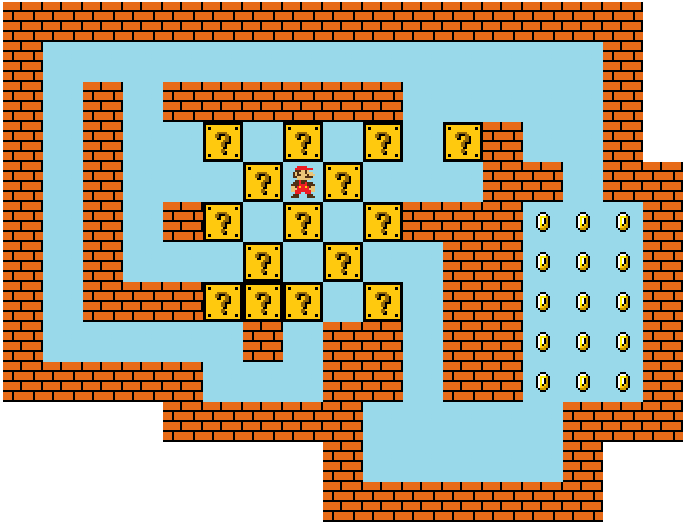
\includegraphics[width=0.617\textwidth]{teste8}
	\caption[]{\small\sl Teste F.9}
	\captionsetup[figure]{list=no}
\end{figure}

\begin{figure}[h]
	\centering
	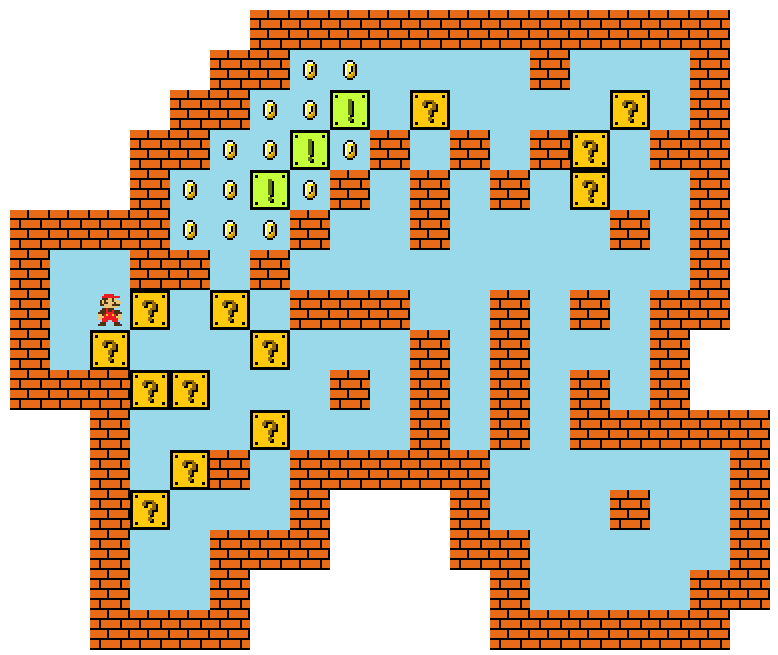
\includegraphics[width=0.75\textwidth]{teste9}
	\caption[]{\small\sl Teste F.10}
	\captionsetup[figure]{list=no}
\end{figure}







\chapter {Conclusões}

A partir do problema inicial, procuramos de todas as formas encontrar uma solução viável para resolver cada uma das tarefas propostas. A partir daí foram surgindo outros problemas que após várias tentativas foram na sua maioria resolvidos, outros não infelizmente.

Assim podemos concluir que a linguagem de programação funcional {\sl Haskell} é bastante útil e cria inúmeras possibilidades quando potenciada com a biblioteca {\sl Gloss} e os pacotes que dela derivam. Apesar das potencialidades existentes da linguagem {\sl Haskell}, é ainda assim uma linguagem difícil de trabalhar comparada a outras linguagens que os elementos deste grupo de trabalho já têm conhecimento e acima de tudo é uma linguagem que requer muita atenção ao mais ínfimo detalhe, pois é muito resumida.

As nossas dificuldades focaram-se principalmente na adaptação ao {\sl Gloss}. Enquanto que na Tarefa F foi necessário fazer alguma pesquisa {\it online} em relação às capacidades da biblioteca e como saber aproveitar das mesmas, na Tarefa E tivemos mais dificuldades principalmente em relação a como criar uma função {\footnotesize\tt rotate} que foi a única função que não conseguimos concluir.

A partir dos nossos erros e daqueles que conseguimos corrigir conseguimos chegar ao resultado final, concluindo assim que o {\sl Haskell} é uma boa linguagem para criar jogos básicos em 2D quando auxiliados com o {\sl Gloss} e será certamente uma escolha no nosso futuro escolar e profissional quando nos for proposto um desafio semelhante a este.





\lstlistoflistings

\listoffigures

\end{document}